% !Mode:: "TeX:UTF-8"

\BiChapter{深度学习辅助词嵌入方法}{}
词嵌入是一种将词语映射为实数向量的技术,这种技术是词语相似度计算中的常用技术。因为相比于词语,向量的相似度比较是非常容易的,通过余弦相似度和平方欧氏距离等方法都可以轻而易举的计算向量的相似度。本章将会介绍一种词嵌入的训练方法,并利用这种方法得到的词嵌入结果计算词语相似度。

词嵌入的训练方法分为直接训练和间接训练。直接训练利用语料库中的统计规律进行训练,最终以得到词嵌入结果为目的;而间接训练则将词嵌入的结果作为其他任务的输入,并将词嵌入矩阵作为模型参数与其他任务的模型共同训练。对于直接训练而言,现在已经有多种成熟的技术,例如NNLM\citeup{Bengio2003}、LBL\citeup{Mnih2007}、C\&W\citeup{Collobert2008}、CBOW\citeup{Mikolov2013}、Skip-gram\citeup{Mikolov2013}与GloVe\citeup{Pennington2014}。而间接训练则多用于深度学习这类基于梯度下降的学习方法中,在第\ref{s:classifer rnn}小节中,本课题就使用了一种间接训练的方式来训练词嵌入。

上述的直接训练方法都是通过词语与其上下文间的关系来进行训练的,这些方法分为两个类型。其中一种(NNLM、LBL、CBOW、Skip-gram)认为,一个词语应该可以被其上下文所预测出来。而一种该方法(C\&W)认为,应该存在一个打分函数,使得一个词语与其上下文之间的得分尽可能高。除此之外,这些方法还使用不同的方式来组合上下文词语\citeup{Lai2016}。

本章介绍的词嵌入方法是一种直接训练的方法。它将会利用深度学习的技术,对LBL的一种改进方法ivLBL\citeup{Mnih2013}进行了改进。

\BiSection{原理介绍}{}
\BiSubsection{ivLBL}{}
\label{s:ivlbl}
由于本章介绍的方法是基于ivLBL方法的改进,所以在这里首先介绍ivLBL方法\footnote{实际上,为了更好的介绍本章的模型,本小节的内容与原文\citeup{Mnih2013}介绍的ivLBL模型有一定偏差。原文使用了上下文词语间的独立假设,对本小节介绍的部分又进行了更加深入的改进。这一部分将不在本文的讨论范围之内。}。

沿用公式\ref{e:corpus}中对于$\mathcal{C}$的定义,设有一个词语$w \in \mathcal{V}$,我们很容易从语料库中找到包含这个词语的一个句子$s$,该句子满足$s \in \mathcal{C}, s_i = w$。目标词语附近一定范围内的词语(除自身外)称为称为这个词语的上下文。即:
\begin{equation}
c = (s_l, \dots, s_{i - 1}, s_{i + 1}, \dots, s_r), 1 \leq l \leq i \leq r \leq |s|, l \neq r
\end{equation}

与其他基于上下文预测的词嵌入方法类似,ivLBL方法使用两个词嵌入矩阵$E$与$E'$,分别用于目标词与上下文中的词语的嵌入。这样,目标词$w$的嵌入表示为$E_w$,而上下文中的一个词语$h_i$的嵌入表示为$E'_{h_i}$。

接下来需要根据整个上下文得到一个预测表示。预测表示是一个与$E_w$维度相同的向量。为了完成这个任务,需要一个表示函数$\hat{q}$。在ivLBL中,其定义如下:
\begin{equation}
\hat{q}(c) = \frac{1}{n}\sum_{i = 1}^{|c|}E'_{h_i}
\end{equation}

得到向量表示以后,我们需要一个打分函数$s_\theta$以评价预测向量与实际向量的相似程度。这个函数可以实现为一个简单的线性变换:
\begin{equation}
s_\theta(w, c) = \hat{q}(c)^\intercal E_w + b_w
\label{e:scoring}
\end{equation}

利用这样的打分函数,就可以进行目标词语的预测。

\BiSubsection{上下文表示}{}
上文中介绍了与上下文$c$有关的概念,以及上下文表示函数$\hat{q}$。而本课题使用的方法与ivLBL方法的不同之处就在于这两者。现有的ivLBL方法选择固定并且较短(论文中使用的是10,目标词语前后各5个词语)的上下文长度,这样的长度并不足以挖掘句子中的全部上下文信息。并且ivLBL使用的简单平均方式还会丢失词语的顺序信息。

为了完整照顾整个句子中的所有上下文信息,我们设上下文的范围为整个句子。这样,对于句子$s$中的每一个词语$s_i$,我们都可以得到一个与之对应的上下文$c = (s_1, \dots, s_{i - 1}, s_{i + 1}, \dots, s_{|s|})$。

令$e'_i = E'_{s_i}$,假设我们将$e'_i$组成的序列输入LSTM模型中,这样就可以得到一个输出序列$h_i$。由第\ref{s:classifer lstm}小节的介绍可以得知,输出项$h_{i - 1}$可以携带输入项$e'_1, \dots, e'_{i - 1}$的全部信息,这覆盖了上下文$c$的前半部分。

但是这还不够,因为我们无法覆盖剩余的部分。为了解决这个问题,需要使用双向LSTM。

\BiSubsection{双向LSTM}{}
双向LSTM\citeup{Graves2005}是LSTM模型的一个变种,它分为前向连接和后向连接,其具有如图\ref{f:bidirectional lstm}所示的结构。其前向连接与第\ref{s:classifer lstm}小节中介绍的普通LSTM完全一致,而后向连接则将中间状态的传递方向改为了从$|s|$到$1$。

\begin{figure}[h]
	\centering
	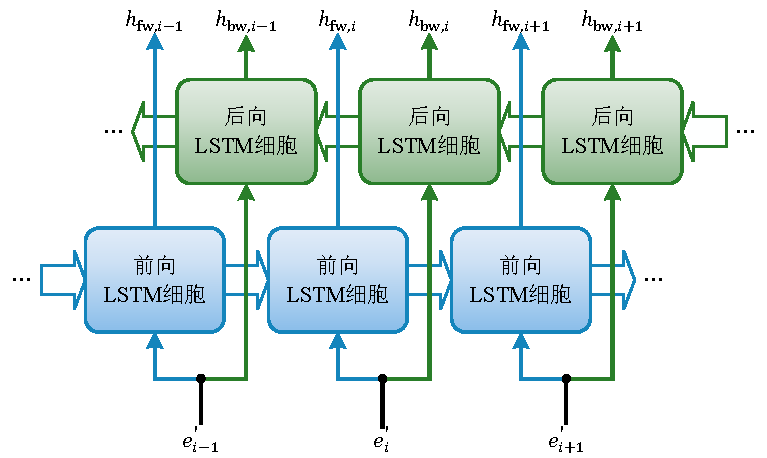
\includegraphics{bidirectional-LSTM}
	\caption{双向LSTM结构}
	\label{f:bidirectional lstm}
	\vspace{-1em}
\end{figure}

双向LSTM中的前向LSTM细胞和后向LSTM细胞是相同形状的LSTM细胞,但它们之间的参数值互相独立,不能共享。$h_\text{fw}$是前向连接的输出,而$h_\text{bw}$是后向连接的输出。双向LSTM的完整定义如公式\ref{e:bilstm begin}--\ref{e:bilstm end}所述。

\begin{align}
	f_{\text{fw}, i} &= \sigma(W_{\text{f}, \text{fw}} e_{\text{fw}, i} + U_{\text{f}, \text{fw}} h_{\text{fw}, i - 1} + b_{\text{f}, \text{fw}}) \label{e:bilstm begin} \\
	f_{\text{bw}, i} &= \sigma(W_{\text{f}, \text{bw}} e_{\text{bw}, i} + U_{\text{f}, \text{bw}} h_{\text{bw}, i + 1} + b_{\text{f}, \text{bw}}) \\
	i_{\text{fw}, i} &= \sigma(W_{\text{i}, \text{fw}} e_{\text{fw}, i} + U_{\text{i}, \text{fw}} h_{\text{fw}, i - 1} + b_{\text{i}, \text{fw}}) \\
	i_{\text{bw}, i} &= \sigma(W_{\text{i}, \text{bw}} e_{\text{bw}, i} + U_{\text{i}, \text{bw}} h_{\text{bw}, i + 1} + b_{\text{i}, \text{bw}}) \\
	o_{\text{fw}, i} &= \sigma(W_{\text{o}, \text{fw}} e_{\text{fw}, i} + U_{\text{o}, \text{fw}} h_{\text{fw}, i - 1} + b_{\text{o}, \text{fw}}) \\
	o_{\text{bw}, i} &= \sigma(W_{\text{o}, \text{bw}} e_{\text{bw}, i} + U_{\text{o}, \text{bw}} h_{\text{bw}, i + 1} + b_{\text{o}, \text{bw}}) \\
	c_{\text{fw}, i} &= f_{\text{fw}, i} \circ c_{\text{fw}, i - 1} + i_{\text{fw}, i} \circ \tanh(W_{\text{c}, \text{fw}} e_{\text{fw}, i} + U_{\text{c}, \text{fw}} h_{\text{fw}, i - 1} + b_{\text{c}, \text{fw}}) \\
	c_{\text{bw}, i} &= f_{\text{bw}, i} \circ c_{\text{bw}, i + 1} + i_{\text{bw}, i} \circ \tanh(W_{\text{c}, \text{bw}} e_{\text{bw}, i} + U_{\text{c}, \text{bw}} h_{\text{bw}, i + 1} + b_{\text{c}, \text{bw}}) \\
	h_{\text{fw}, i} &= o_{\text{fw}, i} \circ \tanh(c_{\text{fw}, i}) \\
	h_{\text{bw}, i} &= o_{\text{bw}, i} \circ \tanh(c_{\text{bw}, i}) \label{e:bilstm end}
\end{align}

这样,对于词语$s_i$,$h_{\text{fw}, i - 1}$与$h_{\text{bw}, i + 1}$便分别包含了其上下文$c$前半部分和后半部分的信息。为了得到向量形式的上下文表示$\hat{q}(c)$,还需要将两个向量拼接在一起,并输入一个全连接层:
\begin{equation}
\hat{q}(c) = \tanh\bigl(W_\text{full} [h_{\text{fw}, i - 1}, h_{\text{bw}, i + 1}] + b_\text{full}\bigr)
\end{equation}

\BiSubsection{噪声对比估计}{}
第\ref{s:ivlbl}小节提到,利用公式\ref{e:scoring}中给出的打分函数,就可以进行目标词语的预测。设$p(w \mid c)$是在上下文$c$中出现词语$w$的实际概率,一种非常容易想到的想法是,使用柔性最大值函数对打分函数$s_\theta(w, c)$在整个词汇集上进行规范化,就可以得到对$p(w \mid c)$的一个估计,如公式\ref{e:softmax}所述。

\begin{equation}
p(w \mid c, \theta) = \frac{e^{s_\theta(w, c)}}{\sum_{v \in \mathcal{V}}e^{s_\theta(v, c)}}
\label{e:softmax}
\end{equation}

然而,这样的方法在实际训练中是不现实的。这种方法意味着对于每一个词语$w$,我们都必须对打分函数进行$|\mathcal{V}|$次求值\footnote{在本课题的实际训练中,词汇量达到了$5 \times 10^5$个。},这样的时间复杂度是完全无法接受的。

ivLBL使用了噪声对比估计\citeup{Graves2005}的方法来解决这个问题,这种方法建立了一个辅助的二分类问题。设$w'$是从某种分布中采样得到的随机词语,这种词语被称为“噪声”,则可以生成二分类问题的输入样本及其标记$(v, y)$:
\begin{equation}
y = \begin{cases}
1 & v = w, \\
0 & v = w'
\end{cases}
\end{equation}
在数据生成的过程中,噪声词语的数量是目标词语的$k$倍。这样对于一个词语$v$,其属于目标词语的概率为:
\begin{equation}
p(D = 1 \mid v) = \frac{p(v \mid h)}{p(v \mid h) + k p_\text{noise}(v)}
\end{equation}
其中,$p_\text{noise}(v)$是噪声分布中词语$v$的概率。

对公式\ref{e:scoring}中给出的打分函数应用sigmoid函数,就可以得到对$p(v \mid h)$的一个估计:
\begin{equation}
p(v \mid c, \theta) = \sigma\bigl(s_\theta(v, c)\bigr)
\end{equation}
使用$p(v \mid c, \theta)$代替$p(v \mid h)$,可以得到对$p(D = 1 \mid v)$的估计:
\begin{equation}
p(D = 1 \mid v, \theta) = \frac{p(v \mid c, \theta)}{p(v \mid c, \theta) + k p_\text{noise}(v)} = \sigma\Bigl(\log\bigl(p(v \mid c, \theta)\bigr) - \log\bigl(k p_\text{noise}(v)\bigr)\Bigr)
\end{equation}

由于噪声对比估计模型工作在未规范化的数据集上,因此可以简单用$s_\theta(v, c)$代替$\log\bigl(p(v \mid c, \theta)\bigr)$,于是得到\footnote{由于项$\log\bigl(k p_\text{noise}(v)\bigr)$是与$v$有关的常量,其和$s_\theta(v, c)$中可训练的偏置项$b_v$是直接相加关系。因此本课题简化模型,将二者合并为一个偏置项。}:
\begin{equation}
p(D = 1 \mid v, \theta) = \sigma\Bigl(s_\theta(v, c) - \log\bigl(k p_\text{noise}(v)\bigr)\Bigr)
\end{equation}

应用交叉熵损失函数,可以得到:
\begin{equation}
L_{w, \theta} = \log p(D = 1 \mid w, \theta) + \sum_{i = 1}^{k} \log\bigl(1 - p(D = 1 \mid w'_i, \theta)\bigr)
\end{equation}

\BiSubsection{模型训练}{}
训练模型使用的优化算法与第\ref{s:classifer p-training}小节中介绍的完全相同,为Adam算法,这里不再赘述。

\BiSection{程序实现}{}
由于两种方法在技术上的相似性(均以深度学习为主),深度学习辅助词嵌入方法与深度学习的二分类方法使用了相同的程序整体结构。因此,本节的整体结构部分可以完全参照第\ref{s:classifer implementation}节的描述。
\BiSubsection{数据预处理}{}
深度学习辅助词嵌入方法的数据预处理程序结构如图\ref{f:nce preprocess}所示。本次选用的语料库仍然是THUCNews数据集。实际上,“分局分词”、“词典构造”与“查询编号”的部分与第\ref{s:classfier preprocess}小节是完全相同的,其代码也是完全共享。这大大减少了编程的复杂程度。

\begin{figure}[h]
	\centering
	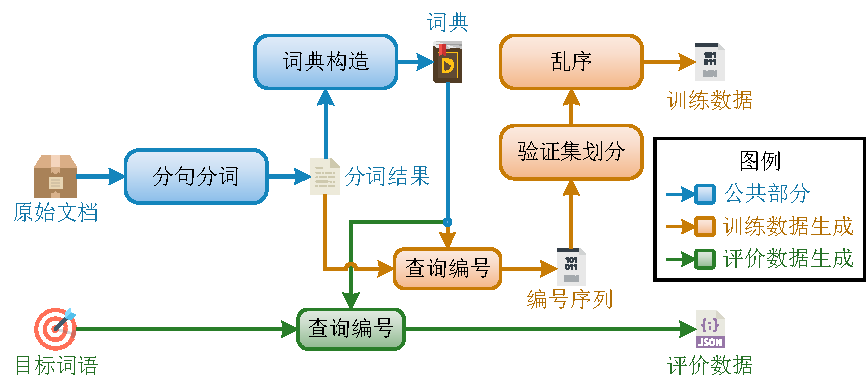
\includegraphics{NCE-preprocess}
	\caption{数据预处理}
	\label{f:nce preprocess}
	\vspace{-1em}
\end{figure}

与之前不同的是,由于词嵌入训练直接使用语料库中的句子,因此本小节的数据预处理程序没有采样句生成的部分。词语的编号序列将直接划分为验证集和训练集,并进行乱序。划分和乱序的算法也与第\ref{s:classfier preprocess}小节相同。

由于词语相似度评价需要计算目标词语的词嵌入间的相似度,因此也需要查询目标词语的编号。目标词语编号查询的结果将会保存在JSON文件中。

\BiSubsection{模型训练}{}
模型训练过程除所构建的TensorFlow图与第\ref{s:classifer training}小节不同外,其余内容全部相同,本小节不再赘述。

\BiSubsection{模型评价}{}
模型评价的程序也是使用Python语言的TensorFlow平台编写的。但是由于输出词语相似度结果不需要训练阶段构建的神经网络,而仅需要从词嵌入矩阵中提取向量,模型评价部分无法复用训练阶段构建的TensorFlow图。

评价程序首先会从训练阶段得到的最优存档点中恢复嵌入矩阵,然后从数据预处理阶段保存的JSON文件中读取目标词语的编号。编号查询和相似度计算的过程被构建在一个新的TensorFlow图中。程序将每一对词语的编号输入TensorFlow图,从词嵌入矩阵中查询对应的向量,并使用预先定义好的函数计算相似度,最终输出结果。对于包含未登录词的词语对,将会取其它词语相似度的平均值。

为了完善实验的结果,本课题分别尝试使用目标词嵌入矩阵$E$、上下文词嵌入矩阵$E'$与二者之和$E + E'$产生词嵌入,而相似度评价函数则尝试了余弦相似度与平方欧式距离,他们的定义如下:
\begin{align}
\text{sim}_\text{c}(A, B) & = \frac{A \cdot B}{|A| |B|} \\
\text{sim}_\text{e}(A, B) & = -|A - B|^2
\end{align}

\BiSection{实验结果}{}
本章所使用的实验环境与表\ref{t:environment}相同,词嵌入的训练进行了一次,其参数与训练情况如表\ref{t:embedding train}所示,而结果如表\ref{t:embedding result}所示。

\begin{table}[h]
	\caption{实验结果}
	\label{t:embedding train}
	\vspace{0.5em}\centering\wuhao
	\begin{tabular}{ccc}
		\toprule[1.5pt]
		词嵌入维数 & LSTM单元数 & 损失函数值 \\
		\midrule[1pt]
		300 & 128 & 14081.98 \\
		\bottomrule[1.5pt]
	\end{tabular}
\end{table}

\begin{table}[h]
\caption{实验结果}
\vspace{0.5em}\centering\wuhao
\begin{tabular}{ccc}
	\toprule[1.5pt]
	相似度函数 & 词嵌入矩阵 & Spearman等级相关系数 \\
	\midrule[1pt]
	$\text{sim}_\text{c}$ & $E$ & 0.3860 \\
	$\text{sim}_\text{c}$ & $E'$ &  0.3542 \\
	$\text{sim}_\text{c}$ & $E + E'$ & 0.3756 \\
	$\text{sim}_\text{e}$ & $E$ &  0.2017 \\
	$\text{sim}_\text{e}$ & $E'$ & 0.0304 \\
	$\text{sim}_\text{e}$ & $E + E'$ & 0.0943 \\
	\bottomrule[1.5pt]
\end{tabular}
\end{table}

\begin{comment}
\begin{table}[h]
	\caption{实验结果}
	\vspace{0.5em}\centering\wuhao
	\begin{tabular}{cccc}
		\toprule[1.5pt]
		\diagbox{相似度函数}{相关系数}{词嵌入矩阵} & $E$ & $E'$ & $E + E'$ \\
		\midrule[1pt]
		$\text{sim}_\text{c}$ & 0.3860 & 0.3542 & 0.3756 \\
		$\text{sim}_\text{e}$ & 0.2017 & 0.0304 & 0.0943 \\
		\bottomrule[1.5pt]
	\end{tabular}
\end{table}

\begin{table}[h]
	\caption{实验结果}
	\vspace{0.5em}\centering\wuhao
	\begin{tabular}{ccccc}
		\toprule[1.5pt]
		\multicolumn{2}{c}{\multirow{2}{*}{Spearman等级相关系数}} & \multicolumn{3}{c}{词嵌入矩阵} \\
		& & $E$ & $E'$ & $E + E'$ \\
		\midrule[1pt]
		\multirow{2}{*}{相似度函数} & $\text{sim}_\text{c}$ & 0.3860 & 0.3542 & 0.3756 \\
		& $\text{sim}_\text{e}$ & 0.2017 & 0.0304 & 0.0943 \\
		\bottomrule[1.5pt]
	\end{tabular}
\end{table}
\end{comment}